\documentclass[12pt]{article}

\usepackage{mathtools}
\usepackage{blindtext}

\usepackage[margin=1in]{geometry}

\newcommand*{\eu}{e}
\newcommand*{\iu}{i}

\DeclarePairedDelimiter{\bra}{\langle}{\rvert}
\DeclarePairedDelimiter{\ket}{\lvert}{\rangle}
\DeclarePairedDelimiterX{\braket}[2]{\langle}{\rangle}
  {#1\,\delimsize\vert\,\mathopen{}#2}

\usepackage{biblatex}
\addbibresource{report.bib}

\usepackage[hidelinks]{hyperref}

\title{Solving Decoherence Channels on Open Quantum Systems}
\author{David Basoco \and Jack Hetherington \and Davis Rash \and Tim Ross}
\date{November 8, 2023}

\begin{document}
  \maketitle

  \section{Introduction}
  \blindtext

  \section{Applications}
  \blindtext

  \section{Depolarizing and Pauli Channels}
  \blindtext

  \section{Markovian Reservoir Engineering}
  \blindtext

  \section{Amplitude Damping}
  \blindtext

  \section{Trace Distance}
        The goal for the trace distance, is to determine the difference between the expected result and the simulated noise result. We can use that the trace distance is half of the trace of the absolute value of the difference of the two density matrices. \\
        Qiskit allows you to obtain the density matrix for a given quantum circuit fairly easily. However it is impossible to obtain the density matrix for a measured set of results. But, we can obtain an approximate density matrix by calculating the probability of being in a specified state then creating an approximate wave function, which we can then use to create an approximate density matrix. From here we can calculate the trace distance.  

  \section{Results}
  \subsection{Trace Distance}
        We were unable to measure the trace distance for our given set of cases, for the reservoir engineering it was not possible to create a density matrix from the results that matched in dimension of the one generated by the circuit without affecting the results. (Add in stuff on other forms?)

  \begin{figure}
    \centering
    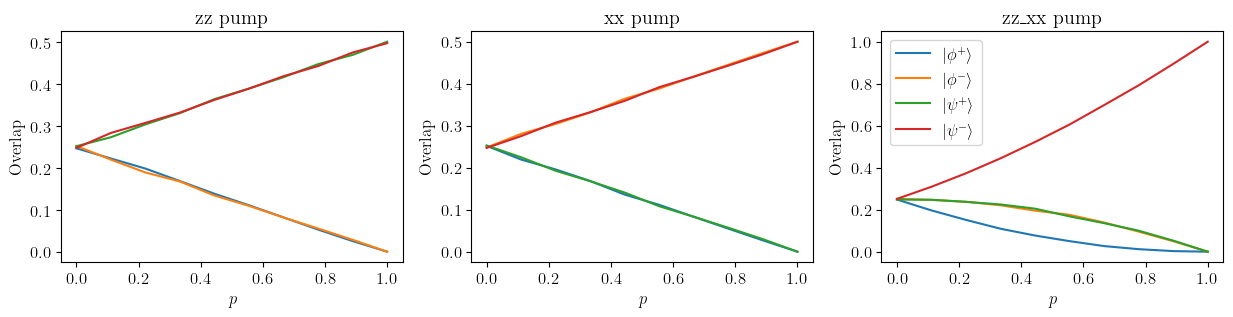
\includegraphics[width=\textwidth]{images/reservoir-engineering-simulation}
    \caption{Simulation of a quantum circuit.%
      \label{fig:reservoir-engineering-simulation}}
  \end{figure}

  \printbibliography
\end{document}